\documentclass{beamer}
\usetheme{Madrid}
\usecolortheme{default}

\usepackage{amsmath}
\usepackage{graphicx}
\usepackage{tikz}
\usetikzlibrary{positioning, shapes.geometric, shapes.misc, arrows.meta, calc}
\usepackage{xcolor}
\usepackage{pgfplots}
\pgfplotsset{compat=1.18}


% ─────────────────────────────────────────────
% COLOR PALETTE
% ─────────────────────────────────────────────
\definecolor{primary}{HTML}{1A6B9A}
\definecolor{secondary}{HTML}{E8F4FD}
\definecolor{accentcol}{HTML}{E87722}
\definecolor{textcol}{HTML}{1E2A35}
\definecolor{mutedcol}{HTML}{6B8A9E}
\definecolor{lightbg}{HTML}{F5F9FC}
\definecolor{bordercol}{HTML}{B8D4E8}
\definecolor{clustblue}{HTML}{2876BD}
\definecolor{clustred}{HTML}{D94F3D}
\definecolor{clustgreen}{HTML}{3A9B6F}

% ─────────────────────────────────────────────
% BEAMER COLORS
% ─────────────────────────────────────────────
\setbeamercolor{palette primary}{bg=primary,fg=white}
\setbeamercolor{palette secondary}{bg=primary!80,fg=white}
\setbeamercolor{palette tertiary}{bg=primary!60,fg=white}
\setbeamercolor{palette quaternary}{bg=primary,fg=white}
\setbeamercolor{structure}{fg=primary}
\setbeamercolor{section in toc}{fg=primary}
\setbeamercolor{frametitle}{bg=primary,fg=white}
\setbeamercolor{title}{bg=primary,fg=white}
\setbeamercolor{background canvas}{bg=lightbg}
\setbeamercolor{block title}{bg=primary,fg=white}
\setbeamercolor{block body}{bg=secondary,fg=textcol}
\setbeamercolor{block title alerted}{bg=accentcol,fg=white}
\setbeamercolor{block body alerted}{bg=accentcol!10,fg=textcol}
\setbeamercolor{block title example}{bg=clustgreen,fg=white}
\setbeamercolor{block body example}{bg=clustgreen!10,fg=textcol}
\setbeamercolor{itemize item}{fg=primary}
\setbeamercolor{itemize subitem}{fg=accentcol}
\setbeamercolor{enumerate item}{fg=primary}

% ─────────────────────────────────────────────
% CUSTOM FRAMETITLE with orange accent stripe
% ─────────────────────────────────────────────
% ─────────────────────────────────────────────
% LOGO ONLY ON TITLE PAGE
% ─────────────────────────────────────────────
\addtobeamertemplate{title page}{}{%
  \begin{tikzpicture}[remember picture,overlay]
    \node[anchor=center, xshift=0cm, yshift=-3.3cm]
      at (current page.center)
      {
\includegraphics[width=1.3cm]{logo.png}};
  \end{tikzpicture}
}


% ─────────────────────────────────────────────
% CUSTOM FOOTLINE  (no author/institute in bar)
% keeps the Madrid short-title | page number look
% ─────────────────────────────────────────────
\setbeamertemplate{footline}{%
  \leavevmode%
  \hbox{%
    \begin{beamercolorbox}[wd=.5\paperwidth,ht=2.25ex,dp=1ex,leftskip=0.4cm]{palette primary}%
      \usebeamerfont{author in head/foot}%
      \color{white}\insertshortinstitute
    \end{beamercolorbox}%
    \begin{beamercolorbox}[wd=.4\paperwidth,ht=2.25ex,dp=1ex,center]{palette secondary}%
      \usebeamerfont{title in head/foot}%
      \color{white}\insertshorttitle
    \end{beamercolorbox}%
    \begin{beamercolorbox}[wd=.1\paperwidth,ht=2.25ex,dp=1ex,right]{palette primary}%
      \color{white}\insertframenumber{}/\inserttotalframenumber\hspace{0.4cm}
    \end{beamercolorbox}%
  }%
}

\setbeamertemplate{itemize item}{\color{primary}\textbullet}
\setbeamertemplate{itemize subitem}{\color{accentcol}$\triangleright$}
\setbeamertemplate{navigation symbols}{}

% ─────────────────────────────────────────────
% TITLE / AUTHOR
% ─────────────────────────────────────────────
\title[K-Means Clustering]{Clustering}
\subtitle{K-Means Clustering Algorithm}

\author[BUET]{%
  \begin{tabular}{ccc}
    \textbf{Anik Gupta} & \textbf{Sourav Sarker} & \textbf{Fardin Fuad} \\[4pt]
    {\small 2205082} & {\small 2205083} & {\small 2205084}
  \end{tabular}
}

\institute[Anik Sourav Fardin, CSE, BUET]{%
  \Large Bangladesh University of Engineering and Technology
}

\date{February 23, 2026}
% ─────────────────────────────────────────────
% TIKZ STYLES — dot = sample, cross = centroid
% ─────────────────────────────────────────────
\tikzset{
  % filled circle = data sample
  sample/.style={circle, fill=#1, draw=#1!80!black,
                 inner sep=0pt, minimum size=5pt, line width=0.4pt},
  % cross-out = centroid
  centroid/.style={cross out, draw=#1, line width=2pt,
                   inner sep=0pt, minimum size=10pt},
  % faded centroid (old position)
  centroid faded/.style={cross out, draw=#1!40, line width=1.2pt,
                          inner sep=0pt, minimum size=10pt},
}

% ─────────────────────────────────────────────
% SHARED PLOT CANVAS macro (saves repetition)
% ─────────────────────────────────────────────
\newcommand{\plotcanvas}{%
  \draw[bordercol, fill=white, line width=1pt]
    (-2.8,-2.2) rectangle (3.6,2.8);
  \foreach \x in {-2,-1,0,1,2,3}
    \draw[bordercol!40, very thin] (\x,-2.2) -- (\x,2.8);
  \foreach \y in {-2,-1,0,1,2}
    \draw[bordercol!40, very thin] (-2.8,\y) -- (3.6,\y);
}

% blue cluster samples
\newcommand{\bluesamples}{%
  \foreach \x/\y in {-1.8/1.8,-1.4/2.0,-1.6/1.4,-2.0/1.6,-1.3/1.2,
                     -1.9/1.0,-1.5/1.6,-1.2/1.8,-2.1/1.3,-1.7/2.2}
    \node[sample=clustblue] at (\x,\y) {};%
}

% red cluster samples
\newcommand{\redsamples}{%
  \foreach \x/\y in {1.8/-0.8,2.2/-0.6,2.0/-1.2,2.5/-0.9,1.6/-1.1,
                     2.3/-1.4,1.9/-0.5,2.6/-1.1,2.1/-1.6,1.7/-0.7}
    \node[sample=clustred] at (\x,\y) {};%
}

% ─────────────────────────────────────────────
\begin{document}
% ─────────────────────────────────────────────

% ══════════════════════════════════════════════
% SLIDE 1 — Title
% ══════════════════════════════════════════════
\begin{frame}
\titlepage
\end{frame}

% ══════════════════════════════════════════════
% SLIDE 2 — Outline
% ══════════════════════════════════════════════
\begin{frame}{Outline}
\tableofcontents
\end{frame}

% ══════════════════════════════════════════════
\section{Introduction to Clustering}
% ══════════════════════════════════════════════

% ──────────────────────────────────────────────
% SLIDE 3 — What is Clustering?
% ──────────────────────────────────────────────
\begin{frame}{What is Clustering?}

\begin{block}{Definition}
An \textbf{unsupervised} learning technique — groups similar data points together without any labels.
\end{block}

\medskip
\begin{columns}[T]
\column{0.52\textwidth}
\textbf{Where is it used?}
\begin{itemize}
  \item Grouping emails or search results
  \item Customer shopping pattern analysis
  \item Segmenting regions of images
\end{itemize}

\bigskip
\textit{Useful when you don't know what patterns exist in your data.}

\column{0.44\textwidth}
\begin{alertblock}{Use With Care}
Can produce \alert{meaningless results} if the wrong distance metric or $K$ is chosen.
\end{alertblock}

\smallskip
\begin{center}
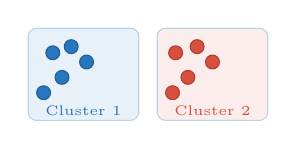
\begin{tikzpicture}[scale=0.78]
  \draw[bordercol,fill=clustblue!10,rounded corners=3pt]
    (-1.7,-0.7) rectangle (0.1,0.8);
  \foreach \x/\y in {-1.3/0.4,-1.0/0.5,-1.15/0.0,-0.75/0.25,-1.45/-0.25}
    \node[sample=clustblue] at (\x,\y) {};
  \draw[bordercol,fill=clustred!10,rounded corners=3pt]
    (0.4,-0.7) rectangle (2.2,0.8);
  \foreach \x/\y in {0.7/0.4,1.05/0.5,0.9/0.0,1.3/0.25,0.65/-0.25}
    \node[sample=clustred] at (\x,\y) {};
  \node[font=\tiny,text=clustblue] at (-0.8,-0.55) {Cluster 1};
  \node[font=\tiny,text=clustred]  at (1.3,-0.55) {Cluster 2};
\end{tikzpicture}
\end{center}
\end{columns}
\end{frame}

% ──────────────────────────────────────────────
% SLIDE 4 — Measuring Similarity
% ──────────────────────────────────────────────
\begin{frame}{Measuring Similarity}

\begin{columns}[T]
\column{0.56\textwidth}
\textbf{One option:} squared Euclidean distance
\[
  \operatorname{dist}(\vec{x},\vec{y}) = \|\vec{x}-\vec{y}\|_2^2
\]

\begin{block}{A Valid Distance Metric Must Satisfy}
\begin{enumerate}\small
  \item \textbf{Symmetry:} $d(x,y)=d(y,x)$
  \item \textbf{Non-negativity:} $d(x,y)\ge 0$
  \item \textbf{Identity:} $d(x,y)=0\Leftrightarrow x=y$
  \item \textbf{Triangle ineq.:} $d(x,z)+d(z,y)\ge d(x,y)$
\end{enumerate}
\end{block}

\column{0.40\textwidth}
\begin{alertblock}{Key Insight}
Clustering results are \alert{crucially dependent} on the chosen similarity measure.
\end{alertblock}

\vspace{0.5cm}
\begin{center}
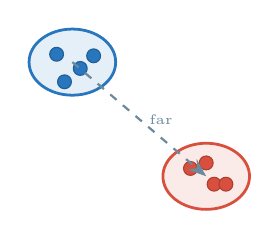
\begin{tikzpicture}[scale=1.0]
  \draw[clustblue,fill=clustblue!12,line width=1pt]
    (-0.85,0.9) ellipse (0.55cm and 0.42cm);
  \draw[clustred,fill=clustred!12,line width=1pt]
    (0.85,-0.55) ellipse (0.55cm and 0.42cm);
  \foreach \x/\y in {-1.05/1.0,-0.75/0.82,-0.95/0.65,-0.58/0.98}
    \node[sample=clustblue] at (\x,\y) {};
  \foreach \x/\y in {0.65/-0.45,0.95/-0.65,0.85/-0.38,1.1/-0.65}
    \node[sample=clustred] at (\x,\y) {};
  \draw[-{Stealth},mutedcol,dashed,line width=0.8pt]
    (-0.85,0.9) -- (0.85,-0.55)
    node[midway,right,font=\tiny,text=mutedcol]{far};
\end{tikzpicture}
\end{center}
\end{columns}
\end{frame}

% ══════════════════════════════════════════════
\section{Clustering Algorithms}
% ══════════════════════════════════════════════

% ──────────────────────────────────────────────
% SLIDE 5 — Types of Clustering
% ──────────────────────────────────────────────
\begin{frame}{Types of Clustering Algorithms}

\begin{columns}[T]
\column{0.48\textwidth}
\begin{minipage}[t][0.72\textheight][t]{\linewidth}
\begin{block}{Partition Algorithms (Flat)}
\begin{itemize}
  \item \textbf{K-Means} — iterative centroid-based
  \item Mixture of Gaussians
  \item Spectral Clustering
\end{itemize}
\end{block}
\vspace{0.3cm}
{\small All points assigned to exactly one of $K$ clusters simultaneously.}
\end{minipage}

\column{0.48\textwidth}
\begin{minipage}[t][0.72\textheight][t]{\linewidth}
\begin{alertblock}{Hierarchical Algorithms}
\begin{itemize}
  \item \textbf{Bottom-up} (agglomerative)\\
        Start with $N$ singletons; merge closest pairs
  \item \textbf{Top-down} (divisive)\\
        Start with one cluster; split recursively
\end{itemize}
\end{alertblock}
\vspace{0.3cm}
{\small Produces a dendrogram of cluster relationships.}
\end{minipage}
\end{columns}

\end{frame}

% ══════════════════════════════════════════════
\section{K-Means Algorithm}
% ══════════════════════════════════════════════

% ──────────────────────────────────────────────
% SLIDE 6 — Algorithm Steps
% ──────────────────────────────────────────────
\begin{frame}{K-Means Algorithm}

\textit{An iterative algorithm that alternates between two simple steps.}

\bigskip
\begin{enumerate}
  \setlength\itemsep{0.4em}
  \item \textbf{Initialize:}   Pick $K$ random points as cluster centroids ($\times$)
  \item \textbf{Alternate:}
        \begin{enumerate}
          \item[\textcolor{primary}{(a)}]
                \textbf{Assign} — each data point ($\bullet$) goes to its nearest centroid
          \item[\textcolor{accentcol}{(b)}]
                \textbf{Update} — move each centroid ($\times$) to the mean of its points
        \end{enumerate}
  \item \textbf{Stop} when no point changes its cluster assignment
\end{enumerate}

\bigskip
\begin{block}{Objective Minimised}
\[
  J \;=\; \sum_{i=1}^{K}\sum_{\vec{x}\in C_i}\|\vec{x}-\vec{\mu}_i\|^2
  \qquad\qquad
  \vec{\mu}_i = \frac{1}{|C_i|}\sum_{\vec{x}\in C_i}\vec{x}
\]
\end{block}

\end{frame}

% ──────────────────────────────────────────────
% SLIDE 7 — Visualise: Initialise
% ──────────────────────────────────────────────
\begin{frame}{K-Means: Step 1 — Initialise ($K=2$)}

\begin{columns}[c]
\column{0.62\textwidth}
\begin{center}
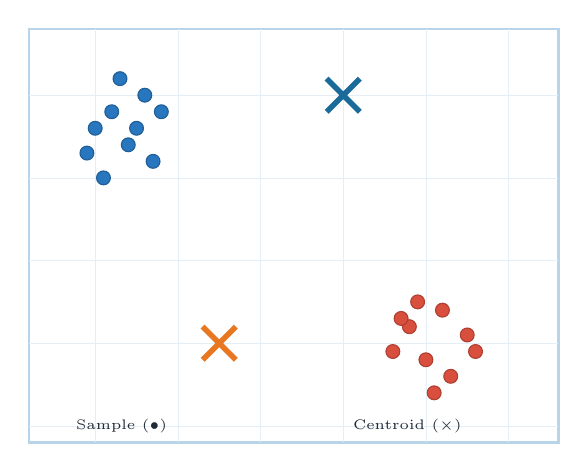
\begin{tikzpicture}[scale=1.05]
  \plotcanvas
  \bluesamples
  \redsamples
  % initial centroids (randomly placed — wrong positions on purpose)
  \node[centroid=primary]   at ( 1.0, 2.0) {};

  \node[centroid=accentcol] at (-0.5,-1.0) {};

  % legend
  % \node[sample=clustblue] at (-2.5,-2.0) {};
  \node[right,font=\tiny,text=textcol] at (-2.35,-2.0) {Sample ($\bullet$)};
  % \node[centroid=primary,minimum size=7pt] at (0.8,-2.0) {};
  \node[right,font=\tiny,text=textcol] at (1.0,-2.0) {Centroid ($\times$)};
\end{tikzpicture}
\end{center}

\column{0.35\textwidth}
\begin{block}{Legend}
  \textbf{$\bullet$} = data sample\\[4pt]
  \textbf{$\times$} = centroid
\end{block}

\medskip
\textbf{$K=2$} centroids are placed \emph{randomly} — they may start far from any real cluster centre.

\medskip
The algorithm will move them iteratively to better positions.
\end{columns}

\end{frame}

% ──────────────────────────────────────────────
% SLIDE 8 — Visualise: Assign
% ──────────────────────────────────────────────
\begin{frame}{K-Means: Step 2a — Assign Samples to Nearest Centroid}

\begin{columns}[c]
\column{0.62\textwidth}
\begin{center}
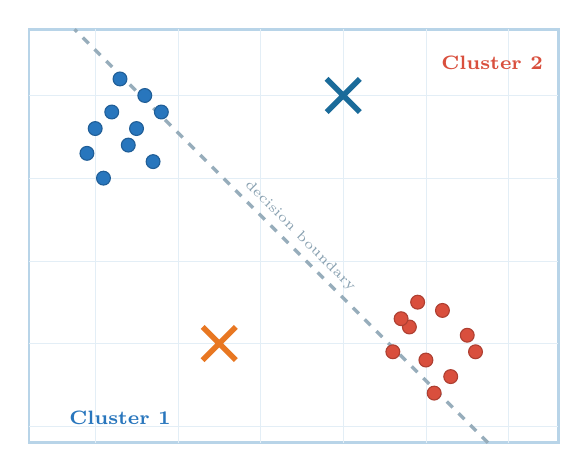
\begin{tikzpicture}[scale=1.05]
  \plotcanvas
  % decision boundary
  \draw[mutedcol!70,dashed,line width=1.2pt]
    (2.75,-2.2) -- (-2.25,2.8);
  \node[font=\tiny,text=mutedcol!80,rotate=315] at (0.48,0.3)
    {decision boundary};
  % samples coloured by nearest centroid
  \bluesamples
  \redsamples
  % centroids (same as step 1)
  \node[centroid=primary]   at ( 1.0, 2.0) {};

  \node[centroid=accentcol] at (-0.5,-1.0) {};

  % cluster labels inside canvas
  \node[font=\scriptsize\bfseries,text=clustblue]  at (-1.7,-1.9) {Cluster 1};
  \node[font=\scriptsize\bfseries,text=clustred]   at ( 2.8, 2.4) {Cluster 2};
\end{tikzpicture}
\end{center}

\column{0.35\textwidth}
Each sample $\bullet$ is coloured by its nearest centroid $\times$.

\medskip
\[d(\bullet,\times_1) \lessgtr d(\bullet,\times_2)\]

\medskip
The dashed line is the \textbf{decision boundary} — equidistant from both centroids.
\end{columns}

\end{frame}

% ──────────────────────────────────────────────
% SLIDE 9 — Visualise: Update Centers
% ──────────────────────────────────────────────
\begin{frame}{K-Means: Step 2b — Update Centroid Positions}

\begin{columns}[c]
\column{0.62\textwidth}
\begin{center}
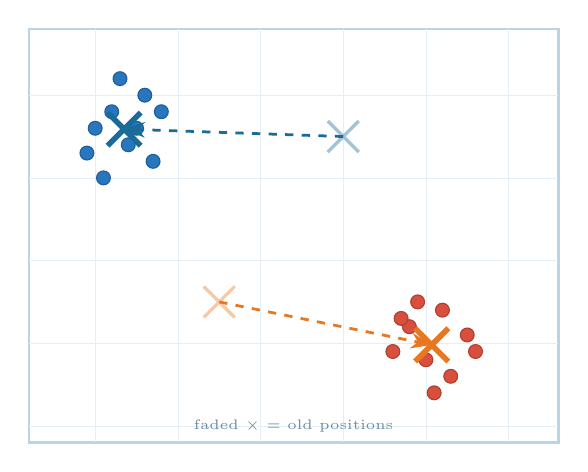
\begin{tikzpicture}[scale=1.05]
  \plotcanvas
  \bluesamples
  \redsamples
  % old centroids (faded)
  \node[centroid faded=primary]   at ( 1.0, 1.5) {};
  \node[centroid faded=accentcol] at (-0.5,-0.5) {};
  % movement arrows
  \draw[-{Stealth},primary,  dashed,line width=1pt]
    (1.0,1.5)   -- (-1.65,1.59);
  \draw[-{Stealth},accentcol,dashed,line width=1pt]
    (-0.5,-0.5) -- ( 2.07,-1.02);
  % new centroids
  \node[centroid=primary]   at (-1.65, 1.59) {};

  \node[centroid=accentcol] at ( 2.07,-1.02) {};

  % note
  \node[font=\tiny,text=mutedcol] at (0.4,-2.0)
    {faded $\times$ = old positions};
\end{tikzpicture}
\end{center}

\column{0.35\textwidth}
Each centroid $\times$ moves to the \textbf{mean} of its assigned samples~$\bullet$.

\medskip
\[
\vec{\mu}_i' = \frac{1}{|C_i|}\!\sum_{\vec{x}\in C_i}\!\vec{x}
\]

\medskip
Faded crosses show the old (bad) positions. Arrows show the movement direction.
\end{columns}

\end{frame}

% ──────────────────────────────────────────────
% SLIDE 10 — Visualise: Convergence
% ──────────────────────────────────────────────
\begin{frame}{K-Means: Convergence}

\begin{columns}[c]
\column{0.62\textwidth}
\begin{center}
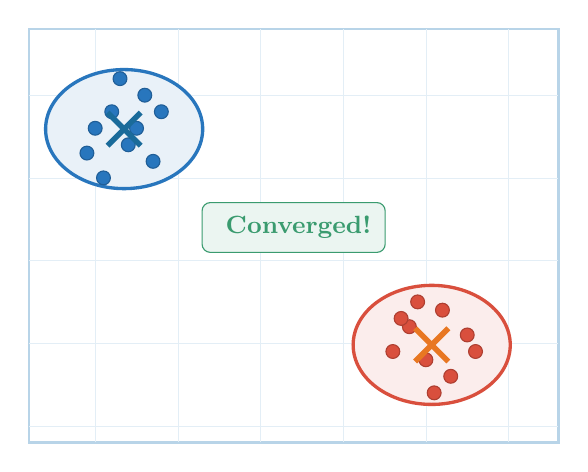
\begin{tikzpicture}[scale=1.05]
  \plotcanvas
  % cluster halos
  \draw[clustblue,fill=clustblue!10,line width=1.2pt]
    (-1.65,1.59) ellipse (0.95cm and 0.72cm);
  \draw[clustred, fill=clustred!10, line width=1.2pt]
    (2.07,-1.02) ellipse (0.95cm and 0.72cm);
  \bluesamples
  \redsamples
  % stable final centroids
  \node[centroid=primary]   at (-1.65, 1.59) {};

  \node[centroid=accentcol] at ( 2.07,-1.02) {};

  % convergence badge
  \node[draw=clustgreen,fill=clustgreen!10,rounded corners=3pt,
        font=\small\bfseries,text=clustgreen,inner sep=5pt]
    at (0.4,0.4) {\checkmark\ Converged!};
\end{tikzpicture}
\end{center}

\column{0.35\textwidth}
No sample changed its cluster — the algorithm has \textbf{converged}.

\medskip
The shaded halos highlight the two final clusters.

\medskip
Centroids $\times$ are now at the \textbf{true centres} of the point clouds.
\end{columns}

\end{frame}

% ══════════════════════════════════════════════
\section{K-Means Properties}
% ══════════════════════════════════════════════

% ──────────────────────────────────────────────
% SLIDE 11 — Properties
% ──────────────────────────────────────────────
\begin{frame}{Properties of K-Means}
  \begin{columns}[T]
    \column{0.48\textwidth}
      \begin{minipage}[t][0.42\textheight][t]{\linewidth}
        \onslide<1->{
        \begin{block}{Running Time per Iteration}
          \begin{enumerate}
            \item Assign samples to nearest centroid: $O(KN)$
            \item Update centroid positions: $O(N)$
          \end{enumerate}
          \textbf{Total per iteration:} $O(KN)$\\
          \textbf{Overall ($I$ iterations):} $O(KNI)$
        \end{block}
        }
      \end{minipage}
      \vspace{0.12cm}
      \begin{minipage}[t][0.42\textheight][t]{\linewidth}
        \onslide<3->{
        \begin{block}{Convergence Guarantee}
          K-means \textbf{always} terminates in a finite number of steps —
          there are finitely many possible assignments.
        \end{block}
        }
      \end{minipage}

    \column{0.48\textwidth}
      \begin{minipage}[t][0.42\textheight][t]{\linewidth}
        \onslide<2->{
        \begin{block}{Objective Function}
          \[ J = \sum_{i=1}^{K}\sum_{\vec{x}\in C_i}\|\vec{x}-\vec{\mu}_i\|^2 \]
          \[ \vec{\mu}_i = \frac{1}{|C_i|}\sum_{\vec{x}\in C_i}\vec{x} \]
        \end{block}
        }
      \end{minipage}
      \vspace{0.12cm}
      \begin{minipage}[t][0.42\textheight][t]{\linewidth}
        \onslide<4->{
        \begin{alertblock}{Local Optimum Only}
          K-means does \alert{not} guarantee the \textbf{global} optimum —
          it converges to a local minimum of $J$.
        \end{alertblock}
        }
      \end{minipage}
  \end{columns}
\end{frame}

% ══════════════════════════════════════════════
\section{Challenges and Considerations}
% ══════════════════════════════════════════════

% ──────────────────────────────────────────────
% SLIDE 12 — Challenges
% ──────────────────────────────────────────────
\begin{frame}{Challenges and Considerations}
  \begin{columns}[T]
    \column{0.48\textwidth}
      \begin{minipage}[t][0.33\textheight][t]{\linewidth}
        \onslide<1->{
        \begin{alertblock}{Initialization Pitfalls}
          \begin{itemize}
            \item Poor start $\Rightarrow$ poor local optimum
            \item Risk of empty clusters
            \item Unbalanced cluster sizes
          \end{itemize}
        \end{alertblock}
        }
      \end{minipage}
      \vspace{0.18cm}
      \begin{minipage}[t][0.33\textheight][t]{\linewidth}
        \onslide<3->{
        \begin{block}{Better Initialization Strategies}
          \begin{itemize}
            \item Multiple random restarts
            \item \textbf{K-means++} — spread initial centroids
            \item Variance-based split / merge
          \end{itemize}
        \end{block}
        }
      \end{minipage}

    \column{0.48\textwidth}
      \begin{minipage}[t][0.33\textheight][t]{\linewidth}
        \onslide<2->{
        \begin{block}{Fundamental Limitations}
          \begin{itemize}
            \item Must specify $K$ in advance
            \item Assumes \textbf{spherical}, convex clusters
            \item Fails on non-convex shapes
          \end{itemize}
        \end{block}
        }
      \end{minipage}
      \vspace{0.18cm}
      \begin{minipage}[t][0.33\textheight][t]{\linewidth}
        \onslide<4->{
        \begin{exampleblock}{When K-Means Fails}
          Concentric rings or crescent \\
          shaped clusters — Euclidean distance cannot separate them correctly.
        \end{exampleblock}
        }
      \end{minipage}
  \end{columns}
\end{frame}

% ══════════════════════════════════════════════
\section{Choosing K — The Elbow Method}
% ══════════════════════════════════════════════

% ──────────────────────────────────────────────
% SLIDE 13 — Elbow Method
% ──────────────────────────────────────────────
\begin{frame}{Choosing $K$ — The Elbow Method}

\begin{columns}[T]
\column{0.42\textwidth}

\textbf{Key Idea:} Run K-means for $K=1,2,\ldots$ and record:
\[
  J(K)=\sum_{i=1}^{K}\sum_{\vec{x}\in C_i}\|\vec{x}-\vec{\mu}_i\|^2
\]
The \textcolor{accentcol}{\textbf{``elbow''}} is where $J$ stops dropping sharply --- that $K$ is optimal.

\smallskip
\textbf{Steps:}
\begin{enumerate}\footnotesize\setlength\itemsep{1pt}
  \item Run K-means for each $K$
  \item Record WCSS
  \item Plot $K$ vs.\ WCSS
  \item Pick the \textcolor{accentcol}{elbow}
\end{enumerate}

\column{0.55\textwidth}
\begin{center}
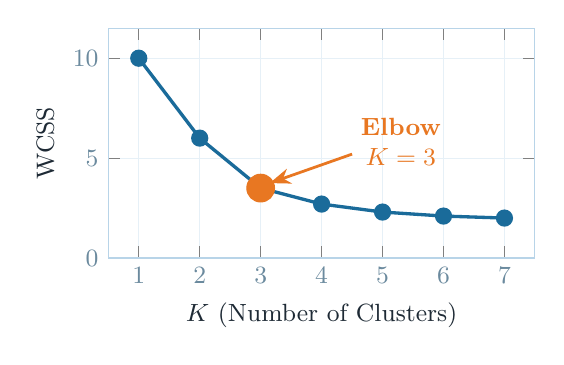
\begin{tikzpicture}
\begin{axis}[
  width=7.0cm, height=4.5cm,
  xlabel={$K$ (Number of Clusters)},
  ylabel={WCSS},
  xtick={1,2,3,4,5,6,7},
  xmin=0.5, xmax=7.5,
  ymin=0,   ymax=11.5,
  grid=both,
  grid style={bordercol!35, very thin},
  axis line style={bordercol, thin},
  tick label style={font=\small, color=mutedcol},
  label style={font=\small, color=textcol},
  axis background/.style={fill=white},
]
  % main WCSS curve (blue dots)
  \addplot[
    primary, very thick,
    mark=*, mark options={fill=primary,draw=primary},
    mark size=2.5pt
  ]
  coordinates {(1,10)(2,6)(3,3.5)(4,2.7)(5,2.3)(6,2.1)(7,2.0)};

  % highlighted elbow point (orange, larger dot)
  \addplot[
    accentcol, only marks,
    mark=*, mark options={fill=accentcol,draw=accentcol},
    mark size=5pt
  ]
  coordinates {(3,3.5)};

  % annotation
  \draw[-{Stealth},accentcol,line width=1pt]
    (axis cs:4.5,5.2) -- (axis cs:3.15,3.75);
  \node[font=\small\bfseries,text=accentcol,align=center]
    at (axis cs:5.3,5.8) {Elbow\\$K=3$};
\end{axis}
\end{tikzpicture}
\end{center}

\begin{alertblock}{\small Note}
\small The elbow can sometimes be ambiguous — always combine with domain knowledge.
\end{alertblock}

\end{columns}
\end{frame}

% ══════════════════════════════════════════════
\section{Applications}
% ══════════════════════════════════════════════

% ──────────────────────────────────────────────
% SLIDE 14 — Applications
% ──────────────────────────────────────────────
\begin{frame}{Applications of K-Means}
  \begin{columns}[T]
    \column{0.48\textwidth}
      \begin{minipage}[t][0.36\textheight][t]{\linewidth}
        \onslide<1->{
        \begin{block}{Image Segmentation}
          \begin{itemize}
            \item Partition image into regions
            \item Colour quantization
            \item Object detection preprocessing
          \end{itemize}
        \end{block}
        }
      \end{minipage}
      \vspace{0.18cm}
      \begin{minipage}[t][0.36\textheight][t]{\linewidth}
        \onslide<3->{
        \begin{block}{Document Clustering}
          \begin{itemize}
            \item Group similar documents
            \item Topic modelling
            \item Search result organisation
          \end{itemize}
        \end{block}
        }
      \end{minipage}

    \column{0.48\textwidth}
      \begin{minipage}[t][0.36\textheight][t]{\linewidth}
        \onslide<2->{
        \begin{alertblock}{Customer Segmentation}
          \begin{itemize}
            \item Market research \& targeting
            \item Personalised recommendations
            \item Behavioural analysis
          \end{itemize}
        \end{alertblock}
        }
      \end{minipage}
      \vspace{0.18cm}
      \begin{minipage}[t][0.36\textheight][t]{\linewidth}
        \onslide<4->{
        \begin{exampleblock}{Gene Expression Analysis}
          \begin{itemize}
            \item Identify gene patterns
            \item Disease classification
            \item Drug discovery research
          \end{itemize}
        \end{exampleblock}
        }
      \end{minipage}
  \end{columns}
\end{frame}
% ══════════════════════════════════════════════
\section{Conclusion}
% ══════════════════════════════════════════════

% ──────────────────────────────────────────────
% SLIDE 15 — Summary
% ──────────────────────────────────────────────
\begin{frame}{Summary}

\begin{itemize}
  \setlength\itemsep{0.45em}
  \item Clustering is an \textbf{unsupervised} learning technique — no labels needed
  \item K-means is simple, efficient, and widely used in practice
  \item Key considerations:
        \begin{itemize}
          \item Choice of $K$ — use the \textcolor{accentcol}{\textbf{Elbow Method}}
          \item Distance metric selection
          \item Initialisation strategy (prefer K-means++)
        \end{itemize}
  \item Hierarchical clustering offers a label-free alternative
  \item Different algorithms suit different data structures
\end{itemize}

\end{frame}

% ──────────────────────────────────────────────
% SLIDE 16 — Key Takeaways
% ──────────────────────────────────────────────
\begin{frame}{Key Takeaways}

\begin{enumerate}
  \setlength\itemsep{0.45em}
  \item K-means \textbf{minimises} within-cluster sum of squares (WCSS)
  \item Convergence is \textbf{guaranteed}, but only to a \alert{local} optimum
  \item Complexity: $O(KNI)$ — $K$ clusters, $N$ points, $I$ iterations
  \item The choice of distance metric is \textbf{crucial}
  \item Use the \textcolor{accentcol}{\textbf{Elbow Method}} to select $K$
  \item Always run \textbf{multiple initialisations} (or use K-means++)
\end{enumerate}

\bigskip
\begin{block}{Elbow Method — Quick Recap}
Plot $K$ vs.\ WCSS and pick the $K$ where the curve stops dropping sharply (the ``elbow''). Diminishing returns beyond that point suggest extra clusters are not meaningful.
\end{block}

\end{frame}

% ──────────────────────────────────────────────
% SLIDE 17 — Thank You  (plain dark slide)
% ──────────────────────────────────────────────
\begin{frame}[plain]

\begin{tikzpicture}[remember picture, overlay]
  % full dark background
  \fill[primary]
    (current page.south west) rectangle (current page.north east);
  % orange accent stripe — top
  \fill[accentcol]
    (current page.north west) rectangle
    ([yshift=-0.22cm]current page.north east);
  % orange accent stripe — bottom
  \fill[accentcol]
    (current page.south west) rectangle
    ([yshift= 0.22cm]current page.south east);
\end{tikzpicture}

\vspace{0.9cm}
\begin{center}
  {\fontsize{44}{50}\selectfont\bfseries\color{white} Thank You!}

  \vspace{0.55cm}
  {\Large\color{white!75!primary} Questions?}

  \vspace{0.45cm}
  {\color{accentcol}\rule{5.5cm}{1.2pt}}

  \vspace{0.5cm}
  {\large\color{white}\bfseries
    Anik Gupta \enspace\textcolor{accentcol}{$\cdot$}\enspace
    Sourav Sarker \enspace\textcolor{accentcol}{$\cdot$}\enspace
    Fardin Fuad}

  \vspace{0.2cm}
  {\small\color{white!65!primary}
    Bangladesh University of Engineering and Technology}
\end{center}

\end{frame}

\end{document}